\documentclass[11pt,a4paper]{article}

% --- Packages ---
\usepackage[utf8]{inputenc}
\usepackage[T1]{fontenc}
\usepackage[english]{babel}
\usepackage{amsmath,amssymb,amsthm}
\usepackage{mathtools}
\usepackage{geometry}
\geometry{margin=2.5cm}
\usepackage{graphicx}
\usepackage{hyperref}
\usepackage{cleveref}
\usepackage{enumitem}
\usepackage{booktabs}
\usepackage{natbib}
\usepackage{xcolor}

% --- Theorem environments ---
\newtheorem{theorem}{Theorem}[section]
\newtheorem{proposition}[theorem]{Proposition}
\newtheorem{lemma}[theorem]{Lemma}
\newtheorem{corollary}[theorem]{Corollary}
\theoremstyle{definition}
\newtheorem{definition}[theorem]{Definition}
\newtheorem{assumption}[theorem]{Assumption}
\newtheorem{remark}[theorem]{Remark}

% --- Cleveref naming for shared theorem counter ---
\Crefname{proposition}{Proposition}{Propositions}
\crefname{proposition}{proposition}{propositions}
\Crefname{lemma}{Lemma}{Lemmas}
\crefname{lemma}{lemma}{lemmas}
\Crefname{remark}{Remark}{Remarks}
\crefname{remark}{remark}{remarks}

% --- Macros ---
\newcommand{\R}{\mathbb{R}}
\newcommand{\N}{\mathbb{N}}
\newcommand{\E}{\mathbb{E}}
\newcommand{\Prob}{\mathbb{P}}
\newcommand{\Q}{\mathbb{Q}}
\newcommand{\Ind}{\mathbf{1}}
\newcommand{\cF}{\mathcal{F}}
\newcommand{\cG}{\mathcal{G}}
\newcommand{\cM}{\mathcal{M}}
\newcommand{\cL}{\mathcal{L}}
\newcommand{\cN}{\mathcal{N}}
\newcommand{\KL}{\mathrm{KL}}
\newcommand{\Ber}{\mathrm{Ber}}

\title{
  \Large\bfseries
  Bayesian Filtering for Interaction-Structure Learning\\
  in Point-Process Interacting Particle Systems
}
\author{
  Marcos Lahoz \and Romain Hû\\[0.5em]
  \small MVA -- Course: Interactions (J.\ Randon-Furling)
}
\date{\today}

\begin{document}
\maketitle

\begin{abstract}
We develop a Bayesian filtering framework for recovering the interaction
structure of a continuous-time Interacting Particle System (IPS) whose
components evolve according to coupled point-process dynamics and are
observed only through their jump times. Instantiating the framework on
a network of stochastic Integrate-and-Fire neurons, we derive the
exact posterior law of the interaction matrix~$W$ under a partial
observation of the spike trains, characterise its dynamics between and
at jumps, and establish posterior consistency, with an explicit
non-asymptotic CLT-based convergence rate in a tractable two-neuron specialisation (with an exogenous Poisson driver) and
a column-wise consistency sketch in the general $n$-neuron case. We factorise the posterior
along incoming edges to reduce the combinatorial burden from~$2^{n(n-1)}$
to~$n\,2^{n-1}$, validate the theory on simulations, and extend the
method to continuous-valued interactions via a Sequential Monte Carlo
particle filter, in line with recent work on nonparametric inference
of interaction laws. The proposed approach complements
targeted-learning and EM-based inference methods discussed in the
course and provides provable statistical guarantees for learning the
structure of interactions in complex systems.
\end{abstract}

% -------------------------------------------------------------------
\section{Introduction}
\label{sec:intro}

Interacting Particle Systems (IPS) are the natural mathematical home for
the phenomena that underpin this course~\citep{Liggett2005,Aldous2013}.
Swarms of animals, agents in a city, synapses in a cortical column,
traders in a limit-order book: each of these can be described as a
collection of elementary units that evolve stochastically and influence
one another through a (typically local) interaction rule. A recurring
theme of the lectures is that the resulting collective dynamics---phase
transitions, consensus, metastability, rare events---are in large part
determined by the \emph{topology and strength of interactions} rather
than by idiosyncratic details of the agents. This makes the inverse
problem of \emph{inferring the interaction structure from observations
of the dynamics} a central one for any data-driven theory of complex
systems.

The inverse problem has been attacked along several orthogonal lines.
Targeted learning~\citep{vanderLaanRose2011} has been applied to recover coupling matrices from equilibrium samples via odds-ratio estimation. Agent-Based Model (ABM)
inference treats the parameters as latent variables and uses an
Expectation--Maximisation or Moment-Matching strategy on
time-aggregated observations~\citep{Banisch2015}. All of these methods operate either in
equilibrium, on coarse-grained observations, or on discrete-time data.
In many natural examples---spike trains of neurons, trades in a market,
contacts in an epidemic---the observations are instead the
\emph{jump times} of a coupled point process, and the identification
must be carried out in continuous time.

\paragraph{This paper.} We propose a Bayesian filtering framework to
address this regime. Our running example is a network of
Integrate-and-Fire neurons with binary or real-valued coupling
matrix~$W$, a canonical point-process IPS. Under a prior on $W$ we
derive closed-form dynamics for the posterior $p_t^w = \Prob(W = w \mid
\cF_t^{N})$ given the observed spikes. We prove posterior consistency
in the large-time limit and quantify the convergence rate through a
Central Limit Theorem on inter-spike log-likelihood ratios. A simple
factorisation along incoming edges collapses the support of the
posterior from $2^{n(n-1)}$ to $n\,2^{n-1}$, which makes the method
computationally feasible on moderate network sizes. We validate
the theory by simulations and extend the framework to continuous $W$
via a bootstrap Sequential Monte Carlo algorithm, demonstrating on a
small example that the filtering perspective survives the discrete-to-
continuous transition.

\paragraph{Position in the ``Interactions'' course.} The paper fits
within Bloc~3 of the course (inference methods) and, through its
continuous-time, spike-train flavour, connects naturally to the
point-process lectures of the companion neuroscience programme.
Compared to the targeted-learning and EM approaches of Lecture~6, our
method requires a stronger assumption---a well-specified generative
model---but in exchange yields (i)~provable consistency, (ii)~explicit
non-asymptotic rates, and (iii)~access to the full posterior rather
than a point estimate, which is useful for uncertainty quantification
and active-experiment design. The Bayesian filter may also be viewed as
a continuous-time, model-based cousin of causal-discovery procedures
\citep{Pearl2009,Manzo2022}: the posterior on~$W$ directly encodes a
distribution over directed interaction graphs.

\paragraph{Contributions.}
\begin{itemize}[itemsep=2pt, topsep=2pt]
  \item We formulate the recovery of the interaction matrix $W$ of a
    point-process IPS as a \emph{nonlinear filtering} problem on the
    partial observation~$\cF_t^{N}$ and derive closed-form evolution
    equations for the posterior, both between and at jumps.
  \item We prove posterior consistency in the large-time limit, with
    an explicit non-asymptotic Berry--Esseen rate via a CLT on the
    inter-spike likelihood ratios in a tractable two-neuron specialisation and a
    column-wise consistency sketch for general $n$.
  \item We exploit a \emph{factorisation by incoming edges} that reduces
    the posterior support from $2^{n(n-1)}$ to $n\,2^{n-1}$, enabling
    computation for moderate network sizes.
  \item We validate the theory by simulations on Erd\H{o}s--R\'enyi
    interaction graphs of sizes $n\,\in\,\{2,3,5,7\}$.
  \item We extend the framework to continuous-valued $W$ via a bootstrap
    Sequential Monte Carlo algorithm, following the line of
    \citet{Lu2019}.
\end{itemize}

\paragraph{Outline.}
\Cref{sec:setup} formulates the model and identifies it as an IPS in
the sense of \citet{Liggett2005}. \Cref{sec:filtering} derives the
filtering equations. \Cref{sec:consistency} proves consistency and
gives a convergence-rate bound. \Cref{sec:nneurons} extends the
analysis to $n$~neurons with the factorised posterior.
\Cref{sec:experiments} reports numerical validation.
\Cref{sec:smc} describes the SMC extension to continuous interactions.
\Cref{sec:discussion} connects the approach to targeted-learning,
ABM inference and causal inference, and outlines directions for future
work.

% -------------------------------------------------------------------
\section{Setup: a point-process IPS with partial observation}
\label{sec:setup}

\subsection{Model}
\label{subsec:model}

Fix $n \geq 2$ and a filtered probability space $(\Omega, \cF,
(\cF_t)_{t \geq 0}, \Prob)$ rich enough to carry all processes below.
For each component $i \in \{1, \ldots, n\}$ we associate a real-valued
hidden state $V_t(i)$ (``potential'') and a counting process $N_t(i)$
(``jumps of~$i$''). The interaction matrix
$W \in \cM_n(\R)$ is random with prior $\pi_0$ and satisfies
$W_{i i} = 0$. Conditionally on~$W$, the pair $(V_t, N_t)_{t \geq 0}$
evolves according to
\begin{equation}
    \mathrm{d} V_t(i) \;=\; \sum_{j \neq i} W_{j i} \,\mathrm{d} N_t(j)
    \;-\; V_{t^-}(i) \,\mathrm{d} N_t(i), \qquad V_0(i) = 0,
    \label{eq:potential}
\end{equation}
and $N_t(i)$ has $\cF_t$-stochastic intensity
\begin{equation}
    \lambda_t(i) \;=\; f\,\bigl( V_{t^-}(i) \bigr),
    \label{eq:intensity}
\end{equation}
where $f \colon \R \to [0, f_{\max}]$ is a bounded smooth intensity
function (e.g. the sigmoid $f(v) = (1 + e^{-v})^{-1}$).
Equation~\eqref{eq:potential} reads: at every jump of neighbour $j$
with $W_{j i} \neq 0$, component $i$ integrates the signed contribution
$W_{j i}$; at every jump of $i$ itself, its state resets to zero.
For the binary case used in most of the
paper, $W \in \{0, 1\}^{n \times n}$ with $W_{i i} = 0$ and we take
$\pi_0 = \Ber(p_{\mathrm{edge}})^{\otimes n(n-1)}$ independent across
edges. The continuous extension considered in~\Cref{sec:smc} replaces
the Bernoulli prior by a Gaussian prior on each~$W_{j i}$.

\subsection{An IPS in Liggett's sense}
\label{subsec:ips}

The process $(V_t, N_t)_{t \geq 0}$ is a pure-jump Markov process on
the Polish state space $\R^n \times \N^n$ with generator, for any
smooth bounded test function $\varphi$ and state $x = (v, k)$,
\begin{equation}
    (\mathcal{A} \varphi)(x) \;=\; \sum_{i=1}^n f(v_i) \bigl[
        \varphi\bigl( T_i(v), k + e_i \bigr) - \varphi(x)
    \bigr],
    \qquad
    T_i(v)_j \;=\; \begin{cases}
        0 & \text{if } j = i, \\
        v_j + W_{i j} & \text{if } j \neq i,
    \end{cases}
    \label{eq:generator}
\end{equation}
where $e_i$ is the $i$-th canonical basis vector of $\R^n$. Locality
is encoded in the support of $W$: only the $i$-th row affects the
$V$-coordinates when $i$ fires, and only the $i$-th column of $W$
determines the potential of~$i$. With $f \equiv \Ind_{[0, \infty)}$
and $W_{j i} \in \{0, 1\}$ one recovers a voter-like process on a
directed graph~\citep{Liggett2005}; with $f$ additionally localised on
the neighbourhood of a site one obtains a contact-process analogue.
Our filtering framework thus applies to a larger family of
point-process IPS than integrate-and-fire networks.

\subsection{Prior and observation}
\label{subsec:prior_obs}

We observe only the full spike-train filtration
$\cG_t \;=\; \sigma\bigl( N_s(i) : s \leq t,\ i = 1, \ldots, n \bigr)$
and seek the posterior
\begin{equation}
    p_t^w \;\coloneqq\; \Prob\bigl( W = w \,\big|\, \cG_t \bigr),
    \qquad w \in \mathrm{supp}(\pi_0).
    \label{eq:posterior_def}
\end{equation}
Neither the potentials~$V_t$ nor the prefactor $W$ are observed.
\Cref{eq:posterior_def} is the classical nonlinear filtering problem
for a marked point process with unknown parameter
\citep{Bremaud1981,Snyder1972,Kallianpur1980}, specialised to a
discrete (resp.\ absolutely continuous) prior on~$W$.

% -------------------------------------------------------------------
\section{Bayesian filtering of the interaction matrix}
\label{sec:filtering}

We first state the filter in the simplest non-trivial case $n = 2$ with
a binary coupling~$J \in \{0, 1\}$, where the posterior reduces to a
one-dimensional stochastic process. The general $n$-neuron treatment is
in~\Cref{sec:nneurons}.

\subsection{Two-neuron model}
\label{subsec:two-neuron}

For tractability we depart slightly from the coupled model of \Cref{sec:setup}: instead of letting neuron~2 fire with intensity $f(V_t(2))$, we replace it by an exogenous Poisson driver of fixed rate~$\theta$. This isolates the unknown coupling $J = W_{2 \to 1}$ and yields a one-dimensional posterior; the coupled $n = 2$ case is recovered as the column-wise specialisation of \Cref{sec:nneurons}. Concretely, let $\widetilde N$ be a Poisson process of rate $\theta > 0$ (exogenous
driver) and set
\begin{equation}
    \mathrm{d} V_t \;=\; J \,\mathrm{d} \widetilde N_t \;-\; V_{t^-}
    \,\mathrm{d} N_t,\qquad V_0 = 0,
    \qquad
    \lambda_t(N) = f(V_{t^-}).
    \label{eq:two-neuron}
\end{equation}
The prior is $\Prob(J = 1) = 1 - p_0 = 1 - \Prob(J = 0)$. Write
$p_t^1 \coloneqq \Prob(J = 1 \mid \cG_t)$ and $V_t^{(j)}$ for the
potential trajectory one would obtain under hypothesis $J = j$. A
Girsanov change-of-measure argument~\citep{Bremaud1981}
yields the filtering equations (sketch in~\Cref{app:filter}):

\begin{proposition}[Two-neuron filter]
\label{prop:filter-2}
On any interval $(\tau_k, \tau_{k+1})$ between consecutive jumps of
either $\widetilde N$ or $N$, the posterior evolves according to
\begin{equation}
    \frac{\mathrm{d} p_t^1}{\mathrm{d} t} \;=\; p_t^1 (1 - p_t^1)
    \bigl[ f(V_t^{(0)}) - f(V_t^{(1)}) \bigr].
    \label{eq:ode-posterior}
\end{equation}
At a jump of the exogenous process $\widetilde N$ the posterior does
not change (both hypotheses predict the jump with the same probability
$\theta \mathrm{d} t$); at a jump of~$N$ at time~$\tau$ the posterior
is updated by Bayes:
\begin{equation}
    p_\tau^1 \;=\; \frac{f\bigl( V_{\tau^-}^{(1)} \bigr) \, p_{\tau^-}^1}
    {f\bigl( V_{\tau^-}^{(0)} \bigr) (1 - p_{\tau^-}^1) +
     f\bigl( V_{\tau^-}^{(1)} \bigr) p_{\tau^-}^1}.
    \label{eq:jump-posterior}
\end{equation}
\end{proposition}

Intuitively, between jumps the
posterior drifts towards the hypothesis whose predicted intensity
$f(V_t^{(j)})$ is smallest, because the absence of a spike is more
consistent with that hypothesis; at a jump the posterior is multiplied by the hypothesis' intensity. Note that this result is obtained as a particular case of the derivation detailed in~\Cref{subsec:nneuron-filter}.

\begin{remark}[Why only jumps of~$N$ matter]
In~\eqref{eq:jump-posterior} only the observed process~$N$ updates the
posterior. This is a general feature of point-process filtering: a
jump of a process whose intensity depends on the unknown parameter is
informative; a jump of a process with parameter-free rate (here
$\widetilde N$ with rate~$\theta$) carries information only through the
subsequent evolution of the potentials $V_t^{(j)}$.
\end{remark}

\subsection{Full $n$-neuron filter}
\label{subsec:nneuron-filter}

In the $n$-neuron model of~\Cref{sec:setup} each column $W_{\cdot, i}$
of $W$ determines the potential of neuron~$i$ but does not appear in
any other potential. Under a product prior
$\pi_0(W) = \prod_{i=1}^n \pi_0^i(W_{\cdot, i})$, the posterior
factorises along columns,
\begin{equation}
    p_t^W \;=\; \prod_{i=1}^n p_t^i(W_{\cdot, i}),
    \label{eq:factorisation}
\end{equation}
and each factor satisfies an analogue of~\eqref{eq:ode-posterior} and
\eqref{eq:jump-posterior} with $V$ replaced by the hypothesis-indexed
potential $V^{(w)}(i)$. We summarise the resulting dynamics in
\Cref{prop:filter-n} below and defer the derivation
to~\Cref{sec:nneurons}.

\begin{proposition}[$n$-neuron filter, factorised form]
\label{prop:filter-n}
Let $p_t^i(w)$ be the posterior mass of the configuration
$w \in \mathrm{supp}(\pi_0^i)$ on the incoming edges of neuron~$i$.
Between jumps,
\begin{equation}
    \frac{\mathrm{d} p_t^i(w)}{\mathrm{d} t} \;=\; p_t^i(w) \Bigl[
        \bar \lambda_t(i) - f\bigl( V_t^{(w)}(i) \bigr) \Bigr],
    \qquad
    \bar \lambda_t(i) \;\coloneqq\; \sum_{w'} p_t^i(w') \,
        f\bigl( V_t^{(w')}(i) \bigr),
    \label{eq:ode-n}
\end{equation}
and at a jump of neuron~$i$ at time~$\tau$, only the factor of
neuron~$i$ is updated:
\begin{equation}
    p_\tau^i(w) \;\propto\; f\bigl( V_{\tau^-}^{(w)}(i) \bigr)
        \, p_{\tau^-}^i(w).
    \label{eq:jump-n}
\end{equation}
Jumps of neighbours $j \neq i$ do not modify $p_t^i$ directly but do
update the hypothesis-indexed potentials $V_t^{(w)}(i)$.
\end{proposition}

\begin{remark}[Consistency with the two-neuron case]
For $n = 2$ the support $\mathrm{supp}(\pi_0^1) = \{0, 1\}$ and
\eqref{eq:ode-n} reduces, after writing $p \coloneqq p_t^1(1) = p_t^1$
and $1 - p = p_t^1(0)$, to $\mathrm{d} p/\mathrm{d} t = p\,[\bar\lambda
- f(V^{(1)})]$ with $\bar\lambda = (1-p) f(V^{(0)}) + p f(V^{(1)})$,
which simplifies to $p(1-p)\,[f(V^{(0)}) - f(V^{(1)})]$, exactly
\eqref{eq:ode-posterior}.
\end{remark}

The key complexity reduction is that
$\mathrm{supp}(\pi_0^i) \subset \{0, 1\}^{n-1}$ has cardinality
$2^{n-1}$ rather than $2^{n(n-1)}$, so the full posterior is stored and
updated in $O(n \cdot 2^{n-1})$ memory. This is the observation that
unlocks the experiments of~\Cref{sec:experiments} for $n$ up to~$7$.

% -------------------------------------------------------------------
\section{Posterior consistency and convergence rate}
\label{sec:consistency}

We now show that the posterior of~\Cref{prop:filter-2} concentrates on
the true value $J^\star$ of~$J$ as $t \to \infty$, and we quantify the
rate of convergence in the number of observed spikes.

\subsection{Identifiability via Kullback--Leibler}
\label{subsec:identifiability}

Denote by $r_t \coloneqq p_t^1 / (1 - p_t^1)$ the posterior odds ratio
and let $\tau_k$ be the time of the $k$-th spike of~$N$ (we index by
spikes of~$N$ rather than by generic events because only these reset
the potentials). A direct computation from \eqref{eq:ode-posterior}--
\eqref{eq:jump-posterior} gives
\begin{equation}
    \log r_{\tau_k} \;=\; \log r_0 \;+\; \sum_{\ell=1}^{k} X_\ell,
    \qquad
    X_\ell \;\coloneqq\; \log \frac{K_1(\xi_\ell)}{K_0(\xi_\ell)},
    \label{eq:random-walk}
\end{equation}
where
$\xi_\ell \coloneqq (V^{(0)}_{\tau_{\ell-1}:\tau_\ell},
V^{(1)}_{\tau_{\ell-1}:\tau_\ell},
\widetilde N_{|(\tau_{\ell-1},\tau_\ell]})$ is the full inter-spike
trajectory on $(\tau_{\ell-1}, \tau_\ell]$---including every jump of the
exogenous driver $\widetilde N$ that occurs in that window---and $K_j$
is its law under hypothesis $J = j$. Since $V^{(j)}_{\tau_\ell} = 0$ at
every spike of $N$ and $\widetilde N$ is a homogeneous Poisson process
independent of the past, the strong Markov property ensures that the
$\xi_\ell$ form an i.i.d.\ sequence under each $K_j$. Consequently
\eqref{eq:random-walk} is a random walk with drift
\begin{equation}
    \E_{J^\star}[X_\ell] \;=\; \begin{cases}
        \phantom{-}\KL(K_1 \| K_0) \;>\; 0 & \text{if } J^\star = 1, \\
        -\KL(K_0 \| K_1) \;<\; 0 & \text{if } J^\star = 0,
    \end{cases}
\end{equation}
the two KL divergences being strictly positive whenever $f(0) \neq
f(1)$ and $\theta > 0$: the first condition ensures that the two
hypotheses give different intensities after at least one jump of
$\widetilde N$, and $\theta > 0$ ensures that such a jump occurs with
positive probability before the next spike of~$N$. Together these are
our identifiability conditions.
The Strong Law of Large Numbers applied
to~\eqref{eq:random-walk} therefore yields~\emph{posterior consistency}:
\begin{equation}
    p_t^{J^\star} \;\xrightarrow[t \to \infty]{\mathrm{a.s.}} \; 1.
    \label{eq:consistency}
\end{equation}

\subsection{CLT-based convergence rate}
\label{subsec:clt}

A more refined analysis yields the speed at which the posterior
concentrates. Define, for $\varepsilon \in (0, 1/2)$, the hitting
time in the event counting
\begin{equation}
    k_\varepsilon \;\coloneqq\; \inf\bigl\{ k \in \N :
        \bigl| p_{\tau_k}^1 - J^\star \bigr| < \varepsilon \bigr\}.
\end{equation}
Let $\mu \coloneqq \E[X_1 \mid J^\star]$ and
$\sigma^2 \coloneqq \mathrm{Var}[X_1 \mid J^\star]$. By the central
limit theorem applied to~\eqref{eq:random-walk}, the rescaled
$\log r_{\tau_k} - k \mu$ is asymptotically Gaussian with variance
$k \sigma^2$. A Berry--Esseen-type approximation gives the following
bound (see~\Cref{app:clt}):
\begin{proposition}[Non-asymptotic convergence rate]
\label{prop:rate}
Assume $J^\star = 1$, take a uniform prior $p_0 = 1/2$ (so that $\log r_0 = 0$), and assume the intensity is bounded both above and below: $0 < f_{\min} \leq f \leq f_{\max}$ (which guarantees $\rho = \E|X_1 - \mu|^3 < \infty$ since $\log f$ stays bounded). Write $A_\varepsilon = \log ((1 - \varepsilon) / \varepsilon)$. Then for every $k \geq 1$,
\begin{equation}
    \Prob\bigl( k_\varepsilon \leq k \bigr) \;\geq\;
    \Phi\!\left( \frac{k \mu - A_\varepsilon}{\sigma \sqrt{k}} \right)
    \;-\; \frac{C \rho}{\sigma^3 \sqrt{k}},
\end{equation}
where $\Phi$ is the standard normal cdf and $C$ is the absolute constant from
the Berry--Esseen inequality. Equivalently, as $\varepsilon \downarrow
0$, the smallest $k$ guaranteeing $\Prob(k_\varepsilon \leq k) \geq
1 - \delta$ satisfies
\begin{equation*}
    k \;=\; \frac{A_\varepsilon}{\mu}
    \;+\; z_{1-\delta}\,\frac{\sigma\,\sqrt{A_\varepsilon / \mu}}{\mu}
    \;+\; o\!\left(\sqrt{A_\varepsilon}\right),
\end{equation*}
so the leading term $A_\varepsilon/\mu$ is a Kullback--Leibler
commitment time and the $O(\sqrt{A_\varepsilon})$ correction is a
Gaussian fluctuation.
\end{proposition}
We validate~\Cref{prop:rate} numerically in~\Cref{sec:experiments}.

% -------------------------------------------------------------------
\section{Extension to $n$ neurons and factorised posterior}
\label{sec:nneurons}

We now give the $n$-neuron generalisation of~\Cref{prop:filter-2}
together with the factorisation that underlies the algorithm used in
the experiments. We start by deriving the general equation driving the posterior between jumps.

\subsection{General posterior ODE}
\label{subsec:general-ode}

In the general case, we consider a network of neurons whose potentials are driven by the following SDE:
$$
dV_t^i = -V_{t-}^i\, dN_t^i + \sum_{j \neq i} w_{j i}\, dN_t^j
$$
where $N_t^i$ is a point process with predictable intensity $f(V_{t-}^i(w))$ associated to neuron $i$ and $w$ is the connectivity matrix. The Girsanov likelihood in this general case is given by

$$
L_t (w) = \prod_i \prod_{k:\,\tau_k^i \le t} f\bigl(V_{\tau_k^i-}^i (w)\bigr)\, \exp \left( -\int_0^t f(V_s^i (w))\, ds \right)
$$

Finally, the change of measure formula for Poisson processes yields the explicit formula for the posterior:
$
p_t(w) = \frac{L_t(w) p_0 (w)}{\mathbb{E}_{p_0}[L_t (w)]} = \frac{q_t (w)}{\sum_{w'} q_t (w')}
$
with prior $p_0$ over connectivity matrices.

Differentiating this formula in time between spikes yields the ODE satisfied by the posterior:
\begin{align*}
    \dot{p}_t (w) &= \frac{\dot{q}_t (w) \sum_{w'} q_t (w') - q_t (w) \sum_{w'} \dot{q}_t (w')}{\left( \sum_{w'} q_t (w') \right)^2} \\
    &= \frac{-q_t (w) \sum_i f(V_t^i (w)) \sum_{w'} q_t (w') + \sum_{w'} q_t(w') \sum_i f(V_t^i (w')) q_t(w)}{\left( \sum_{w'} q_t (w') \right)^2} \\
    &= \frac{-q_t(w) \Lambda_t (w) Z_t + \sum_{w'} q_t(w') \Lambda_t (w') q_t(w)}{Z_t^2} \\
    &= \frac{q_t(w)}{Z_t^2} \left( -\Lambda_t(w) Z_t + \sum_{w'} q_t(w') \Lambda_t (w') \right) \\
    &= \frac{q_t (w)}{Z_t} \left( -\Lambda_t(w) + \sum_{w'} \frac{q_t(w')}{Z_t} \Lambda_t (w') \right) \\
    &= p_t (w) \left( \sum_{w'} p_t (w') \Lambda_t (w') - \Lambda_t(w) \right) \\
    &= p_t(w) \left( \mathbb{E}_{p_t}[\Lambda_t (w)] - \Lambda_t(w) \right)
\end{align*}

Specifying this formula in the two-neuron case recovers the earlier formula of~\Cref{subsec:two-neuron}. Note that this formula extends naturally to real-valued $w$.

At spikes of neuron $i$, the posterior update stems directly from the change of measure formula:
$$
p_{\tau_k^i} (w) = \frac{f(V_{\tau_k^i-}^i (w)) p_{\tau_k^i-} (w)}{\mathbb{E}_{p_{\tau_k^i-}}[f(V_{\tau_k^i-}^i (w'))]}
$$

\subsection{Full and factorised posterior}

Let $\pi_0$ be a prior on $W \in \{0, 1\}^{n \times n}$ with
$W_{i i} = 0$ almost surely. The naive posterior
$p_t^w = \Prob(W = w \mid \cG_t)$ is supported on
$2^{n(n-1)}$ configurations. The following observation, central to our
method, makes the problem tractable.

\begin{lemma}[Column-wise factorisation]
\label{lem:factorisation}
Under~\eqref{eq:potential}, the potential $V_t(i)$ depends on $W$ only
through its $i$-th column $W_{\cdot, i}$, so the likelihood of the
observation $\cG_t$ factorises as
\begin{equation}
    \cL\bigl( \cG_t \mid W \bigr) \;=\; \prod_{i=1}^n
        \cL_i\bigl( N(i) \mid W_{\cdot, i} \bigr),
    \label{eq:lik-factorisation}
\end{equation}
where $\cL_i$ is the likelihood of the spike train of neuron~$i$
conditional on the incoming edges $W_{\cdot, i}$. Consequently, if
$\pi_0 = \prod_i \pi_0^i$ is a product prior, the posterior is also
a product and \eqref{eq:factorisation} holds.
\end{lemma}

\begin{proof}
Integrating~\eqref{eq:potential} over any interval between jumps
of~$N(i)$ gives $V_t(i) = \sum_{j \neq i} W_{j i}\,\Delta N_t^{(i)}(j)$
where $\Delta N^{(i)}(j)$ counts the spikes of~$j$ since the last
reset of~$i$. Hence $V(i)$ (and thus $\lambda(i) = f(V(i))$)
only involves $W_{\cdot, i}$. The likelihood of a point process with
compensator $\int_0^t \lambda_s \mathrm{d} s$ factors as
$\exp(-\int \lambda) \prod f(V_{\tau-})$ (see, e.g., Thm~2 of
Chapter~II.3 of~\citealp{Bremaud1981}), giving~\eqref{eq:lik-factorisation}.
Bayes' rule then yields~\eqref{eq:factorisation}.
\qed
\end{proof}

\Cref{lem:factorisation} cuts the memory from $2^{n(n-1)}$ to
$n \cdot 2^{n-1}$. The derivation of \Cref{prop:filter-n} is obtained
by applying the two-neuron filter within each column separately, the
only subtle point being the propagation of the hypothesis-indexed
potentials $V_t^{(w)}(i)$: at a jump of neighbour~$j$ at time~$\tau$,
every candidate~$w$ has its potential incremented by $w_j$ (the bit
of~$w$ at position~$j$). This is exactly the book-keeping carried out
in the simulator of~\Cref{sec:experiments}.

\subsection{Consistency (sketch)}

The consistency argument of~\Cref{subsec:identifiability} extends
columnwise. By~\Cref{lem:factorisation}, the posterior factorises
along columns, so it is enough to prove consistency separately for
each column. Fix neuron~$i$ and let $w^\star \in \{0, 1\}^{n-1}$ be
the true incoming-edge configuration of neuron~$i$ (i.e.\ the $i$-th
column of $W^\star$). Write $q_t^i(w) \coloneqq L_t^i(w)\,p_0^i(w)$ for the unnormalised posterior mass of column $w$ on neuron~$i$, where $L_t^i$ is the per-column likelihood of~\Cref{lem:factorisation}, and let $r_t^{w, w^\star}(i) \coloneqq \log \frac{q_t^i(w)}{q_t^i(w^\star)}$ denote the log-likelihood ratio between $w$ and $w^\star$ along the spike train of neuron~$i$. A direct computation gives
\begin{equation}
    r_t^{w, w^\star}(i) \;=\; \int_0^t \log \frac{f(V_s^i(w))}{f(V_s^i(w^\star))}\, dN_s^i + \int_0^t \bigl[ f(V_s^i(w^\star)) - f(V_s^i(w)) \bigr]\, ds + \log \frac{p_0^i(w)}{p_0^i(w^\star)},
\end{equation}
where $p_0^i$ is the marginal prior on the $i$-th column.

By the Doob--Meyer decomposition of $N^i$ under~$\Prob_{w^\star}$
(whose compensator is $\int_0^t f(V_s^i(w^\star))\,ds$), we can rewrite
\[
r_t^{w, w^\star}(i) \;=\; \int_0^t \left[ \log \frac{f(V_s^i(w))}{f(V_s^i(w^\star))}\, f(V_s^i(w^\star)) +  f(V_s^i(w^\star)) - f(V_s^i(w)) \right] ds + \log \frac{p_0^i(w)}{p_0^i(w^\star)} + M_t,
\]
where $M_t$ is a martingale whose predictable quadratic variation $\langle M\rangle_t$ is bounded above by $C\, t$ (since $f$ is bounded above and $\log f$ is bounded on the relevant range). By the strong law of large numbers for square-integrable martingales (Kolmogorov-type, since $\langle M\rangle_t/t^2 \to 0$), $M_t/t \to 0$ a.s. Dividing by~$t$, the contributions
$M_t/t$ and $\tfrac{1}{t}\log p_0^i(w)/p_0^i(w^\star)$ vanish as
$t \to \infty$, leaving
\[
H_t \;=\; \frac{1}{t} \int_0^t \left[ \log \frac{f(V_s^i(w))}{f(V_s^i(w^\star))}\, f(V_s^i(w^\star)) +  f(V_s^i(w^\star)) - f(V_s^i(w)) \right] ds.
\]
The integrand has the form $\Phi(x, y) = y \log \tfrac{x}{y} + y - x$
with $x = f(V_s^i(w))$ and $y = f(V_s^i(w^\star))$. One checks that
$\Phi(x,y) \leq 0$ for all $x, y > 0$, with equality iff $x = y$. Thus
$H_t$ accumulates strictly negative mass on every time interval where
$f(V_s^i(w)) \neq f(V_s^i(w^\star))$.

To turn this into a divergence of $r_t^{w, w^\star}(i)$ to $-\infty$
for $w \neq w^\star$, it suffices to exhibit events on which the two
potentials disagree and to show that such events occur a positive
fraction of the time. Pick any $j$ with $w_j \neq w^\star_j$ and define,
for $\delta > 0$ and $k \geq 1$, the event $E_k^\delta$ as the
conjunction of:
\begin{itemize}
  \item[\textbf{(A)}] neuron~$i$ does not fire in $[\tau_k^i, \tau_k^i + \delta]$;
  \item[\textbf{(B)}] exactly one neighbour from $\mathcal{D} \coloneqq \{j' : w_{j'} \neq w^\star_{j'}\}$ fires in $[\tau_k^i, \tau_k^i + \delta/2]$ (call it $j$);
  \item[\textbf{(C)}] no neighbour from $\mathcal{D}$ fires in $(\tau_k^i + \delta/2, \tau_k^i + \delta]$.
\end{itemize}
At time $\tau_k^i$, neuron~$i$ fires, so $V^i_{\tau_k^i+}(w) = V^i_{\tau_k^i+}(w^\star) = 0$ for \emph{every} configuration (the reset is parameter-independent). Let $\sigma$ denote the time of the unique spike from $\mathcal{D}$ in $[\tau_k^i, \tau_k^i + \delta/2]$ (whose existence is guaranteed by (B), and whose uniqueness rules out cancellations between disagreeing neighbours). Just after $\sigma$, the two potentials differ by exactly $w_j - w^\star_j \neq 0$. By (C), no further spike from $\mathcal{D}$ occurs in $(\sigma, \tau_k^i + \delta]$; spikes of indices outside $\mathcal{D}$ add the same value to both potentials and hence preserve the gap. Combined with (A) (no reset of neuron~$i$), this implies $V^i_s(w) - V^i_s(w^\star) = w_j - w^\star_j \neq 0$ for all $s \in [\sigma, \tau_k^i + \delta]$, hence $f(V_s^i(w)) \neq f(V_s^i(w^\star))$ for a duration at least $\delta/2$. The same construction extends, with minor modifications, to the real-valued case.

Under the standing assumption $f \leq f_{\max}$, the probability that
neuron~$i$ does not fire in a window of length $\delta$ is at least
$\exp(-f_{\max}\delta) > 0$, and the analogous Poisson-rate bounds for
neuron~$j$ give $\Prob(E_k^\delta) \geq c(\delta) > 0$. Provided $f$ is
in addition bounded below by some $f_{\min} > 0$ (so that the
inter-spike times of $N^i$ have finite mean), the strong Markov
property at the spikes of $N^i$ ensures that the average number of
such events up to time~$t$ grows linearly in~$t$ by the law of large
numbers. Combining this with the strict negativity of the
integrand on $E_k^\delta$ yields $H_t \to -c < 0$ a.s., hence
$r_t^{w, w^\star}(i) \to -\infty$ a.s.\ for every $w \neq w^\star$, and therefore $p_t^i(w^\star) \to 1$ a.s. A union bound over the finitely many $w \in \{0,1\}^{n-1} \setminus \{w^\star\}$ preserves almost sure convergence; combined with the column-wise factorisation~\eqref{eq:factorisation}, this gives consistency of the full posterior.

\begin{remark}[Sigmoid intensity]
The sigmoid $f(v) = (1 + e^{-v})^{-1}$ used in our experiments tends to $0$ as $v \to -\infty$ and therefore violates the $f \geq f_{\min} > 0$ assumption underlying the LLN step above. In practice the resets at spikes of neuron~$i$ keep $V^i$ in a bounded regime, and the empirical results of~\Cref{sec:experiments} confirm that consistency holds. A fully rigorous treatment for unbounded-below intensities would require an ergodicity assumption on $V^i$ in the spirit of~\citet{Cormier2020} and is the subject of ongoing work.
\end{remark}

% -------------------------------------------------------------------
\section{Numerical experiments}
\label{sec:experiments}

We now test the filtering framework on simulated data. All experiments
use the sigmoid intensity $f(v) = (1 + e^{-v})^{-1}$, thinning upper
bound $f_{\max} = 1$, and the exact algorithm implied
by~\Cref{prop:filter-n}: between jumps we integrate the ODE
\eqref{eq:ode-n} with an Euler scheme of step $\mathrm{d} t = 10^{-2}$
(checked to be stable); at each accepted spike of neuron~$i$ we apply
the multiplicative update~\eqref{eq:jump-n}. Source code (in Python,
NumPy only) and commands to reproduce every figure are provided in the
companion repository.

\subsection{Two-neuron posterior trajectories}

\Cref{fig:fig1} shows $20$ Monte-Carlo trajectories of the posterior
$p_t^1 = \Prob(J = 1 \mid \cG_t)$ in the two-neuron model of
\Cref{subsec:two-neuron}, for $J^\star \in \{0, 1\}$, with uniform
prior $p_0 = 1/2$ and $\theta = 1$. The pointwise average over
trajectories (red) converges to the ground-truth $J^\star$ within about
$t \approx 100$ time units, in agreement
with~\eqref{eq:consistency}. The individual runs display the expected
path-dependence: trajectories that spike early (hence aggregate
likelihood mass quickly) commit early to the truth, while rare runs
that spike late exhibit a long plateau near the prior before
eventually converging.

\begin{figure}[t]
    \centering
    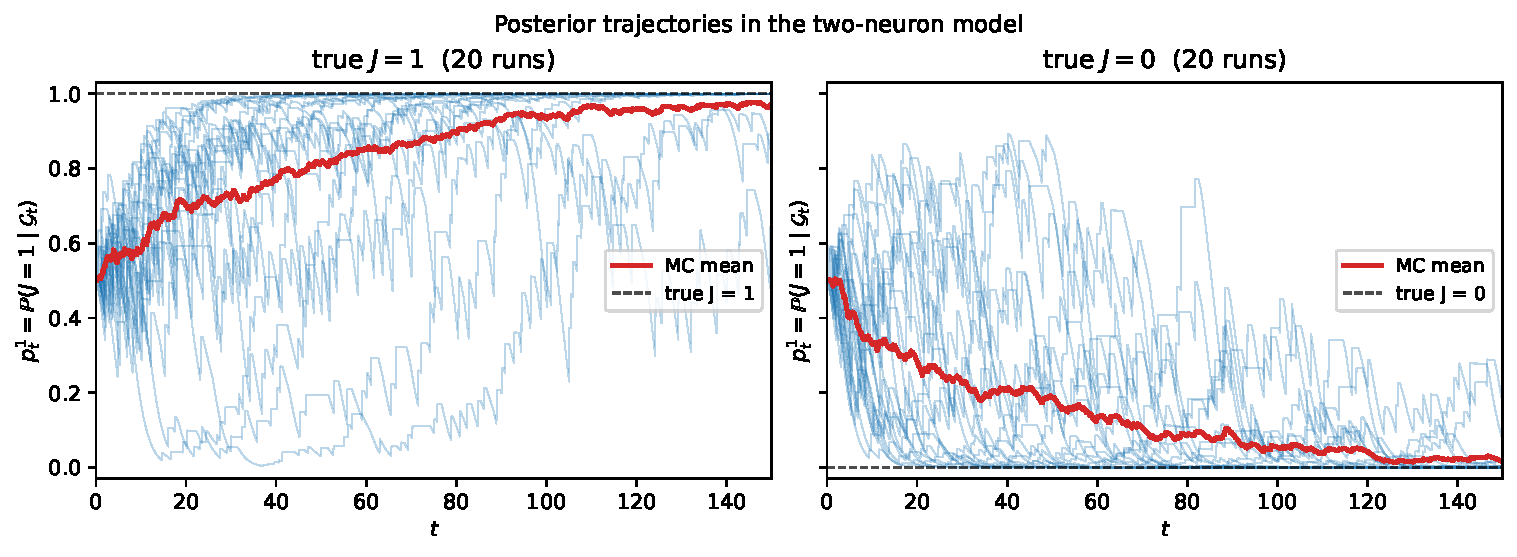
\includegraphics[width=0.92\linewidth]{../code/figures/fig1_posterior_n2.pdf}
    \caption{Posterior trajectories $p_t^1 = \Prob(J = 1 \mid \cG_t)$
    in the two-neuron model. Left: ground truth $J^\star = 1$; right:
    $J^\star = 0$. Grey-blue lines are $N = 20$ individual MC
    replicates; red is their pointwise mean. Convergence to the truth
    is almost sure by~\eqref{eq:consistency}.}
    \label{fig:fig1}
\end{figure}

\subsection{Empirical convergence rate}

\Cref{fig:fig2} validates~\Cref{prop:rate}. Panel~(a) plots the log
posterior-odds $\log r(\tau_k)$ as a function of event count $k$ for
$N = 40$ replicates under each hypothesis. The dashed lines show the
predicted drifts $\pm \KL(K_1 \| K_0)$, with $\KL$ estimated on
$5000$ i.i.d.\ inter-event trajectories. The empirical slopes match
the theoretical ones to within Monte-Carlo noise. Panel~(b) compares
the empirical cumulative distribution of the hitting time
$k_\varepsilon$ (with $\varepsilon = 0.1$) to the CLT approximation of
\Cref{prop:rate}; agreement is excellent despite the modest
number of replicates. Numerical estimates gave
$\hat\mu \approx 0.074$ and $\hat\sigma^2 \approx 0.103$, giving a
characteristic commitment scale of
$k^\star \approx A_\varepsilon / \hat\mu \approx 30$ spikes, in line
with the figure.

\begin{figure}[t]
    \centering
    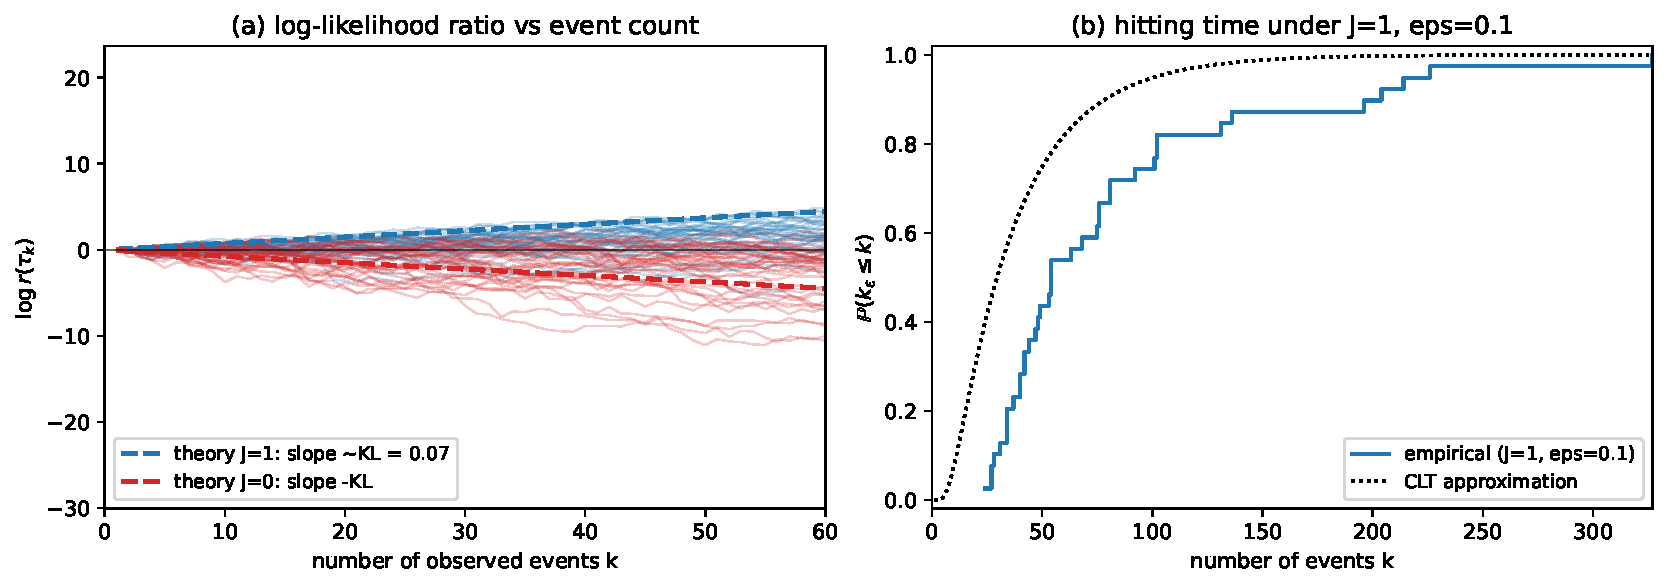
\includegraphics[width=0.92\linewidth]{../code/figures/fig2_convergence_rate.pdf}
    \caption{(a) Log-likelihood ratio $\log r(\tau_k)$ versus event
    count for $N = 40$ replicates under $J^\star = 1$ (blue) and
    $J^\star = 0$ (red), together with the theoretical slopes
    $\pm \KL(K_1 \| K_0)$ (dashed). (b) Empirical CDF of the hitting
    time $k_\varepsilon$ (step, blue) with $\varepsilon = 0.1$ versus
    the CLT approximation of \Cref{prop:rate} (dotted, black).}
    \label{fig:fig2}
\end{figure}

\subsection{Multi-neuron recovery}

We next run the factorised filter on a network of $n = 5$ neurons with
$W^\star$ sampled from $\Ber(0.4)$ i.i.d.\ per edge.
\Cref{fig:fig3} shows the ground-truth coupling matrix, the prior
(uniform $1/2$), and the posterior mean
$\E[W_{j i} \mid \cG_t]$ at intermediate time $t = T/4$ and at the
final time $T = 1500$. The posterior correctly polarises to $\{0, 1\}$
at every off-diagonal entry, with a final Frobenius error of
$\lVert \hat W - W^\star \rVert_F \approx 0.41$ on a matrix of
Frobenius norm $\sqrt{n(n-1) p_{\mathrm{edge}}}$. Residual fuzziness
is concentrated on edges of neurons with low spike rates, for which
identifiability is slower (cf.\ the KL calculation in
\Cref{subsec:identifiability}).

\begin{figure}[t]
    \centering
    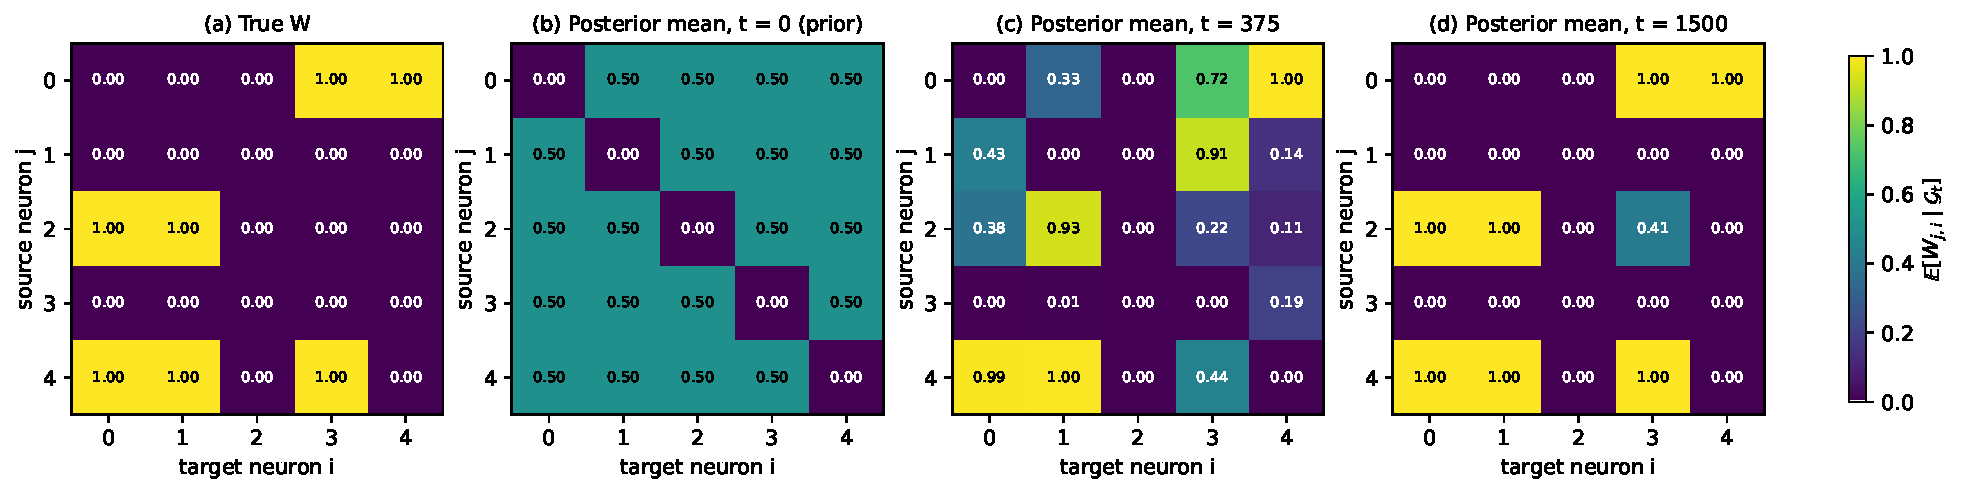
\includegraphics[width=\linewidth]{../code/figures/fig3_posterior_n5.pdf}
    \caption{Recovery of $W$ for $n = 5$. (a)~Ground truth.
    (b)~Uniform prior at $t = 0$. (c)~Posterior mean at $t = T/4$.
    (d)~Posterior mean at $t = T$. Numbers inside each cell are
    $\E[W_{j i} \mid \cG_t]$.}
    \label{fig:fig3}
\end{figure}

\subsection{Scaling of the recovery error}

\Cref{fig:fig4} shows the time-evolution of the normalised Frobenius
error
\[
    e(t) \;\coloneqq\; \lVert \E[W \mid \cG_t] - W^\star \rVert_F
        / \sqrt{n(n-1)}
\]
for $n \in \{3, 5, 7\}$ and $3$ i.i.d.\ replicates each (different
$W^\star$ and different seeds). Bigger networks require longer
observations, both because the number of edges grows like $n^2$ and
because the individual firing rates decrease at fixed prior edge
probability. The curves nevertheless exhibit the same qualitative
shape: a transient plateau during which the first few spikes are
aggregated, followed by a regime where the error decays roughly like
$1 / \sqrt{t}$, consistent with the CLT prediction of
\Cref{prop:rate}.

\begin{figure}[t]
    \centering
    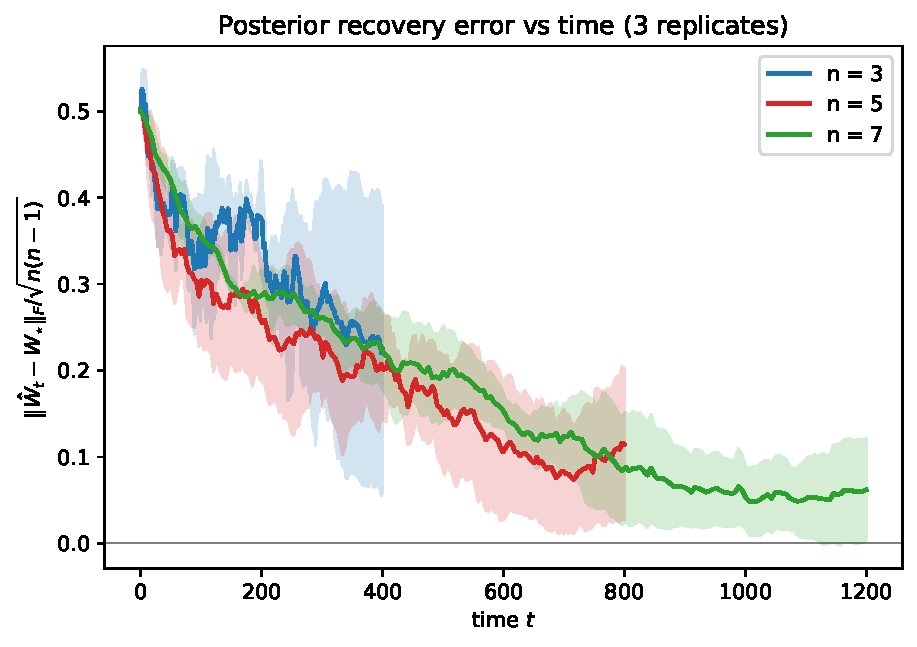
\includegraphics[width=0.7\linewidth]{../code/figures/fig4_error_vs_T.pdf}
    \caption{Mean $\pm$ standard deviation of the normalised Frobenius
    recovery error
    $\lVert \hat W_t - W^\star \rVert_F / \sqrt{n(n-1)}$ across
    $3$ MC replicates, for $n \in \{3, 5, 7\}$. All replicates show
    the expected long-time decay of the posterior error.}
    \label{fig:fig4}
\end{figure}

% -------------------------------------------------------------------
\section{Extension: continuous-valued interactions via SMC}
\label{sec:smc}

The binary constraint $W_{j i} \in \{0, 1\}$ is convenient for
pedagogy but restrictive: in many applications the interaction
strengths are graded, and the inverse problem is intrinsically
infinite-dimensional~\citep{Lu2019}. When the prior on $W$ admits a
Lebesgue density, the posterior~$p_t$ is no longer supported on a
finite set and the exact filter of~\Cref{prop:filter-n} becomes
intractable. We propose here a simple \emph{bootstrap particle filter}
\citep{DoucetGodsillAndrieu2000,ChopinPapaspiliopoulos2020} that
demonstrates, as a proof of concept, that the filtering perspective
survives the discrete-to-continuous transition.

\subsection{Bootstrap particle filter}

We focus on the two-neuron model of~\Cref{subsec:two-neuron} with
$J \in \R$ and Gaussian prior $J \sim \cN(\mu_0, \sigma_0^2)$. The
algorithm maintains $M$ weighted particles $(J^{(m)}, w^{(m)})$; each
particle also tracks its own potential~$V^{(m)}$ driven by the
observed jumps of~$\widetilde N$ and~$N$, because $V$ depends
on~$J$. Writing $t_{k-1}, t_k$ for two consecutive events and noting
that $V^{(m)}$ is constant between events, the likelihood contributed
by that inter-event interval is, for each particle,
\begin{equation}
    \Delta \log w_k^{(m)} \;=\;
    -\,(t_k - t_{k-1})\, f\bigl( V_{t_{k-1}}^{(m)} \bigr)
    \;+\; \Ind\{\text{event is a spike of $N$}\}
        \cdot \log f\bigl( V_{t_k^-}^{(m)} \bigr),
    \label{eq:smc-logw}
\end{equation}
and in between the $V^{(m)}$'s are updated by $V^{(m)} \mathrel{+}=
J^{(m)}$ at each jump of~$\widetilde N$ and reset to zero at each jump
of~$N$. The effective sample size is monitored and whenever it falls
below $M/2$ we resample with replacement and apply a small Gaussian
jitter $J^{(m)} \leftarrow J^{(m)} + \sigma_k \epsilon_m$, with
$\sigma_k = \sigma_0 \cdot (1 + k)^{-\alpha/2}$ and $\alpha \in (0, 1)$
small. This is a static-parameter analogue of the perturbation trick
of~\citet{LiuWest2001} and ensures asymptotic unbiasedness
\citep[Ch.~17]{ChopinPapaspiliopoulos2020}. Details, including the
pseudocode, are given in the accompanying module \texttt{smc.py}.

\subsection{Proof-of-concept experiment}

\begin{figure}[t]
    \centering
    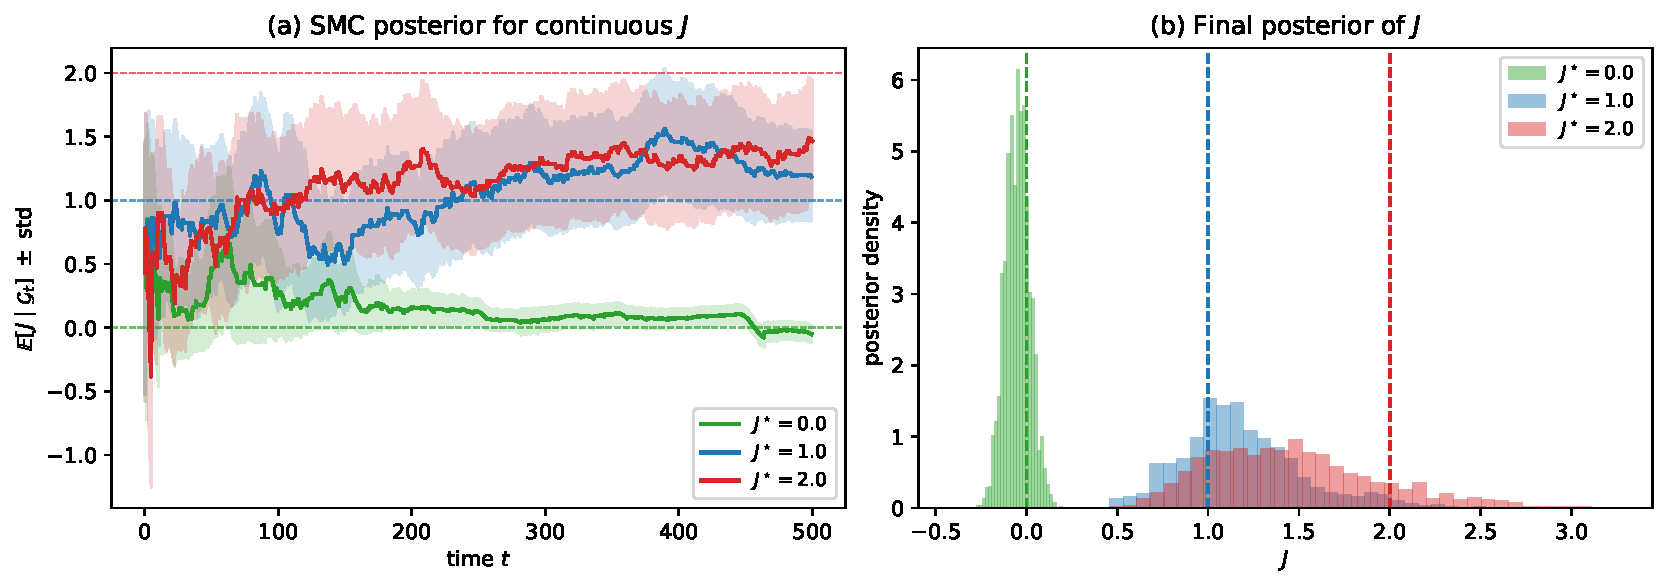
\includegraphics[width=\linewidth]{../code/figures/fig5_smc_continuous.pdf}
    \caption{Bootstrap SMC with $M = 2000$ particles on the two-neuron
    model with continuous $J$, for ground-truth values
    $J^\star \in \{0, 1, 2\}$. (a) Posterior mean $\pm$ standard
    deviation over time; dashed lines mark the respective $J^\star$.
    (b) Final posterior histograms at $T = 500$.}
    \label{fig:fig5}
\end{figure}

\Cref{fig:fig5} reports the posterior mean and std of~$J$ over time as
the filter processes the observed spike train, for three ground-truth
values $J^\star \in \{0, 1, 2\}$. With $M = 2000$ particles, prior
$\cN(0.5, 1)$ and $T = 500$, the posterior concentrates sharply on
$J^\star = 0$ and reasonably on $J^\star = 1$. For $J^\star = 2$ the
filter underestimates $J$ systematically: this is not a bug but a
\emph{saturation effect} of the sigmoid. Since $f(v) \to 1$ as
$v \to \infty$, any $J \gtrsim 2$ produces nearly indistinguishable
likelihoods whenever $V_t \geq 2$, hence the likelihood ridge extends
to arbitrarily large~$J$ and the posterior inherits an almost flat
tail (visible in the right histogram). This is a feature shared by any
unidentifiable parameter: the Bayesian filter reports genuine
uncertainty rather than a misleadingly sharp point estimate, which is
arguably the correct behaviour.

Two directions to scale the SMC to the $n$-neuron setting deserve
mention. First, the column-wise factorisation of
\Cref{lem:factorisation} still holds for continuous $W$, so one may
run $n$ independent SMC filters of dimension $n-1$ each rather than a
single filter of dimension $n(n-1)$. Second, static-parameter
degeneracy can be further mitigated with SMC$^2$ or marginalised
particle filters~\citep{ChopinJacob2013} or with amortised variational
posteriors over $W$. We leave these to future work.

\subsection{Interacting particle filter}
In this subsection, we justify theoretically the use of a different particle filter based on interacting particles. The algorithm is as follows:
\begin{itemize}
    \item at $t = 0$, sample $M$ particles in the search space according to a prior distribution $p_0$. Each particle $(w^1, \ldots, w^M)$ is equipped with a Poisson clock $N_t^m$ with intensity $\sum_i f(V_t^i (w^m)) = \Lambda_t (w^m)$ ;

    \item when $N_t^m$ fires, particle $w_t^m$ is replaced by particle $w_t^{m'}$, with $m'$ sampled uniformly among the particle indices~$\{1,\ldots,M\}$;

    \item at a jump of neuron $i$, each particle $w^m$ is independently redrawn from the categorical distribution that puts mass $f(V_{\tau_k^i-}^i(w^{m'}))/\sum_{m''} f(V_{\tau_k^i-}^i(w^{m''}))$ on $w^{m'}$, for $m' \in \{1,\ldots,M\}$.
\end{itemize}

This algorithm has the advantage of reducing the variance of the posterior by rapidly removing low-likelihood particles. However, it incurs the risk of losing good particles prematurely from the random selection mechanisms. Future work will aim to combine this algorithm with likelihood based SMC methods to get the best of both worlds. Gradient based methods could also be included to provide these algorithms with some exploration abilities.

\subsubsection{Generator of the interacting particle filter}
We prove in this section that the generator of the Markov chain defined by the interacting particle filter algorithm converges to the general posterior ODE. To achieve this, we first derive the general posterior ODE in the sense of distributions.

For a probability distribution $p$ and test function $\Phi$, we denote
$$
\mathbb{E}_p[\Phi(w)] = \int \Phi(w) p(w)\, dw = p(\Phi)
$$

Recall the formula for the posterior ODE between spikes
$
p_t (w) = \frac{L_t (w)}{\mathbb{E}_{p_0}[L_t(w)]}
$

In weak form, this formula becomes
$$
p_t (\Phi) = \frac{\mathbb{E}_{p_0}[\Phi(w) L_t (w)]}{\mathbb{E}_{p_0}[L_t(w)]} = \frac{p_0(\Phi L_t)}{p_0(L_t)} = \frac{\gamma_t(\Phi)}{\gamma_t(1)}
$$

Between spikes, the time derivatives of the unnormalised quantities are $\dot\gamma_t(\Phi) = -\gamma_t(\Lambda_t \Phi)$ and $\dot\gamma_t(1) = -\gamma_t(\Lambda_t)$. The quotient rule then yields
\begin{align*}
    \dot{p}_t(\Phi) &= \frac{\dot{\gamma}_t (\Phi)\, \gamma_t(1) - \gamma_t (\Phi)\, \dot{\gamma}_t (1)}{\gamma_t(1)^2} \\
    &= -\frac{\gamma_t(\Lambda_t \Phi)\, \gamma_t(1) - \gamma_t (\Phi)\, \gamma_t(\Lambda_t)}{\gamma_t(1)^2} \\
    &= -\frac{\gamma_t(\Lambda_t \Phi)}{\gamma_t(1)} + \frac{\gamma_t (\Phi)\, \gamma_t(\Lambda_t)}{\gamma_t(1)^2} \\
    &= p_t(\Phi)\, p_t(\Lambda_t) - p_t(\Lambda_t \Phi).
\end{align*}

At a jump of neuron $i$, the update in weak form writes
$$
p_{\tau_k^i}(\Phi) = \frac{p_{\tau_k^i-}(f(V_{\tau_k^i-}^i(w)) \Phi)}{p_{\tau_k^i-}(f(V_{\tau_k^i-}^i(w)))}
$$

We now turn to the particle filter equations. Let $W = (w^1, \ldots, w^M)$
denote the population vector. The generator of the particle filter
$\mathcal{L}$ splits into a continuous-time component
$\mathcal{L}_\text{cont}$ and a jump component
$\mathcal{L}_\text{spike}$:
\begin{align*}
    \mathcal{L}_\text{cont} \Phi(W) &= \sum_m \Lambda(w^m)\, \frac{1}{M} \sum_{m'} \bigl[\Phi(W^{m \to m'}) - \Phi(W)\bigr], \\
    \mathcal{L}_\text{spike} \Phi(W) &= \sum_i f(V^i(w^\star)) \int \bigl[\Phi(\tilde W) - \Phi(W)\bigr] \prod_m q^i_W(d \tilde w^m),
\end{align*}
where $w^\star$ is the true (latent) connectivity matrix driving the
observed spikes (so neuron~$i$ fires at rate $f(V^i(w^\star))$),
$W^{m \to m'}$ is the population vector with $w^m$ replaced by $w^{m'}$,
and
\[
  q^i_W(d \tilde w) \;\coloneqq\; \sum_m \delta_{w^m}(d \tilde w)\,
        \frac{f(V^i(w^m))}{\sum_{m'} f(V^i(w^{m'}))}
\]
is the likelihood-reweighted empirical measure for neuron~$i$.
In words: at each spike of the true process driven by $w^\star$, the
$M$ particles are jointly resampled, each $\tilde w^m$ being drawn
independently from $q^i_W$, in line with the algorithm described above.

We apply these generators to the test function
$\Phi(W) = \tfrac{1}{M}\sum_m \phi(w^m) = p^W(\phi)$ defined by the
empirical measure $p^W = \tfrac{1}{M}\sum_m \delta_{w^m}$. For the
continuous part,
\begin{align*}
    \mathcal{L}_\text{cont} p^W(\phi) &= \sum_m \Lambda(w^m)\, \frac{1}{M^2} \sum_{m'} \bigl[\phi(w^{m'}) - \phi(w^m)\bigr] \\
    &= \frac{1}{M^2} \left[ \sum_m \Lambda(w^m) \sum_{m'} \phi(w^{m'}) - M \sum_m \Lambda(w^m)\, \phi(w^m) \right] \\
    &= \left( \frac{1}{M} \sum_m \Lambda(w^m) \right) \left( \frac{1}{M} \sum_m \phi(w^m) \right) - \frac{1}{M} \sum_m \Lambda(w^m)\, \phi(w^m) \\
    &= p^W(\Lambda)\, p^W(\phi) - p^W(\Lambda \phi),
\end{align*}
which recovers the continuous-time posterior ODE.

For the spike part, since $p^{\tilde W}(\phi) = \tfrac{1}{M}\sum_m \phi(\tilde w^m)$ and the $\tilde w^m$ are i.i.d.\ draws from $q^i_W$,
\begin{align*}
    \mathcal{L}_\text{spike} p^W(\phi) &= \sum_i f(V^i(w^\star)) \int \bigl[ p^{\tilde W}(\phi) - p^W(\phi) \bigr] \prod_m q^i_W(d \tilde w^m) \\
    &= \sum_i f(V^i(w^\star)) \left[ \int \phi(\tilde w)\, q^i_W(d \tilde w) - p^W(\phi) \right] \\
    &= \sum_i f(V^i(w^\star)) \left[ \frac{p^W(f(V^i)\, \phi)}{p^W(f(V^i))} - p^W(\phi) \right],
\end{align*}
which recovers the Bayesian spike update of \Cref{prop:filter-n}.
Additional mean-field arguments are required to prove the convergence
of $p^W$ to $p$ as $M \to \infty$, which is left
for upcoming work.


% -------------------------------------------------------------------
\section{Discussion and outlook}
\label{sec:discussion}

\paragraph{Relation to targeted learning.} The interaction-structure
inference problem was discussed in Lecture~6 of the course through the
targeted-learning framework of~\citet{vanderLaanRose2011}, applied to Ising-type couplings via odds-ratio estimation. That approach is agnostic about the dynamics and operates
on equilibrium snapshots. Our filter is complementary: it requires a
fully specified point-process generative model, but in exchange
yields posterior consistency together with explicit non-asymptotic
rates (Eq.~\eqref{eq:random-walk} and~\Cref{prop:rate}), as well as the full
posterior rather than a point estimate. When the dynamics are
well-identified from the first principles of the system (as in spiking
networks or epidemic contacts), our filter provides sharper
uncertainty quantification; when only weak structural assumptions are
available, targeted learning remains the natural tool.

\paragraph{Relation to ABM inference and Expectation--Maximisation.}
Agent-based-model inference (Lecture~6;~\citealp{Banisch2015})
typically treats the interaction parameters as latent and optimises
them by EM on time-aggregated observables. In our setting, the
``E-step'' is replaced by the closed-form filtering formulas of
\Cref{prop:filter-n}, which integrate the continuous-time likelihood
exactly rather than its time-averaged moments; no iteration is needed,
and the posterior is available at every observation time. A related
advantage is the ability to start a new prior at any time without
re-optimising: the filter can be warm-started from its current
posterior, which suggests natural extensions to streaming settings or
online hyperparameter adaptation.

\paragraph{Causal interpretation.} Because $W$ encodes a directed
interaction graph, the posterior $p_t^W$ defines a distribution over
causal structures in the sense of~\citet{Pearl2009}. The filtering
viewpoint therefore provides a continuous-time, model-based route to
causal discovery. We highlight two important caveats discussed in the
course's reading of~\citet{Manzo2022}. First, identifiability of $W$
requires the intensity $f$ to be non-constant over the reachable set
of potentials; a flat $f$ makes $W$ causally underdetermined.
Second, the filter is honest about~unidentifiability (as shown by the
flat posterior tail in~\Cref{fig:fig5} for $J^\star = 2$), which is
a meaningful positive when compared to point-estimate-based methods
that may give misleadingly precise answers.

\paragraph{Connections with rare events (Bloc~4).} The consistency
argument of~\Cref{subsec:identifiability} is a large-deviation-type
statement on the log-likelihood ratio. We conjecture that the
posterior of $W$ obeys a Freidlin--Wentzell-style LDP with rate
function governed by the KL divergences between inter-event laws
across hypotheses, bridging the inference problem with the rare-event
themes of the course. A quantitative statement of this type would
sharpen~\Cref{prop:rate} and connect it to the extreme-event
literature on point processes.

\paragraph{Limitations and future work.} The filter currently assumes
the intensity $f$ to depend only on the immediate past potential of the neuron, and the column-wise consistency sketch of~\Cref{sec:nneurons} additionally assumes $f \geq f_{\min} > 0$, an assumption violated by the sigmoid intensity used in~\Cref{sec:experiments} (see the remark at the end of~\Cref{sec:nneurons}). Extensions to intensity functions with memory kernels (e.g.\ Hawkes
processes) would broaden applicability. Moreover, the current SDE driving the network is relatively simple, and more detailed biological features will almost necessarily be required for robust applications of the model to real data. However, the current SDE can be easily modified in certain ways without altering the core methodology, such as by introducing a potential drift between jumps. The
combinatorial cost $n\cdot 2^{n-1}$ still scales exponentially in~$n$
and therefore caps exact inference at $n \sim 10$; graph-sparsity
priors and variational approximations are natural ingredients for
further scaling. The SMC extension can be embedded in the column-wise
factorisation to handle medium-sized continuous-$W$ networks; a
systematic study of degeneracy and resampling schedules is left for
future work.

\paragraph{Reproducibility.} All figures in the paper can be
reproduced from the accompanying Python code by running the scripts
\texttt{code/experiments/fig\{1,2,3,4,5\}\_*.py}. Runtime on a laptop
is under two minutes in total after caching.

% -------------------------------------------------------------------
\bibliographystyle{plainnat}
\bibliography{references}

\appendix

\section{Sketch of the filter derivation}
\label{app:filter}

Let $\Prob^0$ be a reference measure under which $N$ is a Poisson
process of rate $f_{\max}$ independent of everything else; $J$ and
$\widetilde N$ retain their prior laws. Under $\Prob^0$ the filter is
trivial because $N$ is uninformative. The Radon--Nikodym derivative
between the true law $\Prob^J$ and $\Prob^0$ on $\cG_t$ is the
Dol\'eans--Dade exponential
\begin{equation*}
    L_t^J \;=\; \exp\,\Bigl(
        \int_0^t \log \tfrac{f(V_s^{(J)})}{f_{\max}} \,\mathrm{d} N_s
        \;-\; \int_0^t [f(V_s^{(J)}) - f_{\max}] \,\mathrm{d} s
    \Bigr),
\end{equation*}
which corresponds to thinning the Poisson process with rate
$f_{\max}$ at rate $f(V^{(J)})/f_{\max}$. By the Kallianpur--Striebel
formula,
$p_t^1 = \E^0[L_t^1 \Ind\{J = 1\}] / \E^0[L_t^1 \Ind\{J=1\} +
L_t^0 \Ind\{J=0\}]$, and differentiating in time gives~\eqref{eq:ode-posterior}
between jumps of~$N$ and \eqref{eq:jump-posterior} at jumps of~$N$. Jumps
of~$\widetilde N$ contribute equally to $L_t^1$ and $L_t^0$ (the rate
$\theta$ is independent of $J$) and therefore do not update the
posterior. The complete derivation, including the $n$-neuron case, is
given in~\Cref{subsec:general-ode}.

\section{CLT convergence rate}
\label{app:clt}

The random walk~\eqref{eq:random-walk} has i.i.d.\ centred increments
$X_\ell - \mu$ with finite variance $\sigma^2$. A Berry--Esseen
inequality gives, for every $k \geq 1$,
$
    \sup_{x \in \R} \bigl| \Prob\bigl( (S_k - k \mu)/(\sigma \sqrt k)
    \leq x \bigr) - \Phi(x) \bigr|
    \leq C \rho / (\sigma^3 \sqrt k),
$
with $\rho = \E |X_1 - \mu|^3$ and $C$ an absolute constant.
\Cref{prop:rate} then follows by noting that
$\{k_\varepsilon \leq k\} \supseteq \{S_k \geq A_\varepsilon\}$ under
$J^\star = 1$ (the argument is symmetric for $J^\star = 0$).

\end{document}
